\FloatBarrier

\begin{figure}[h!]
	\centering
	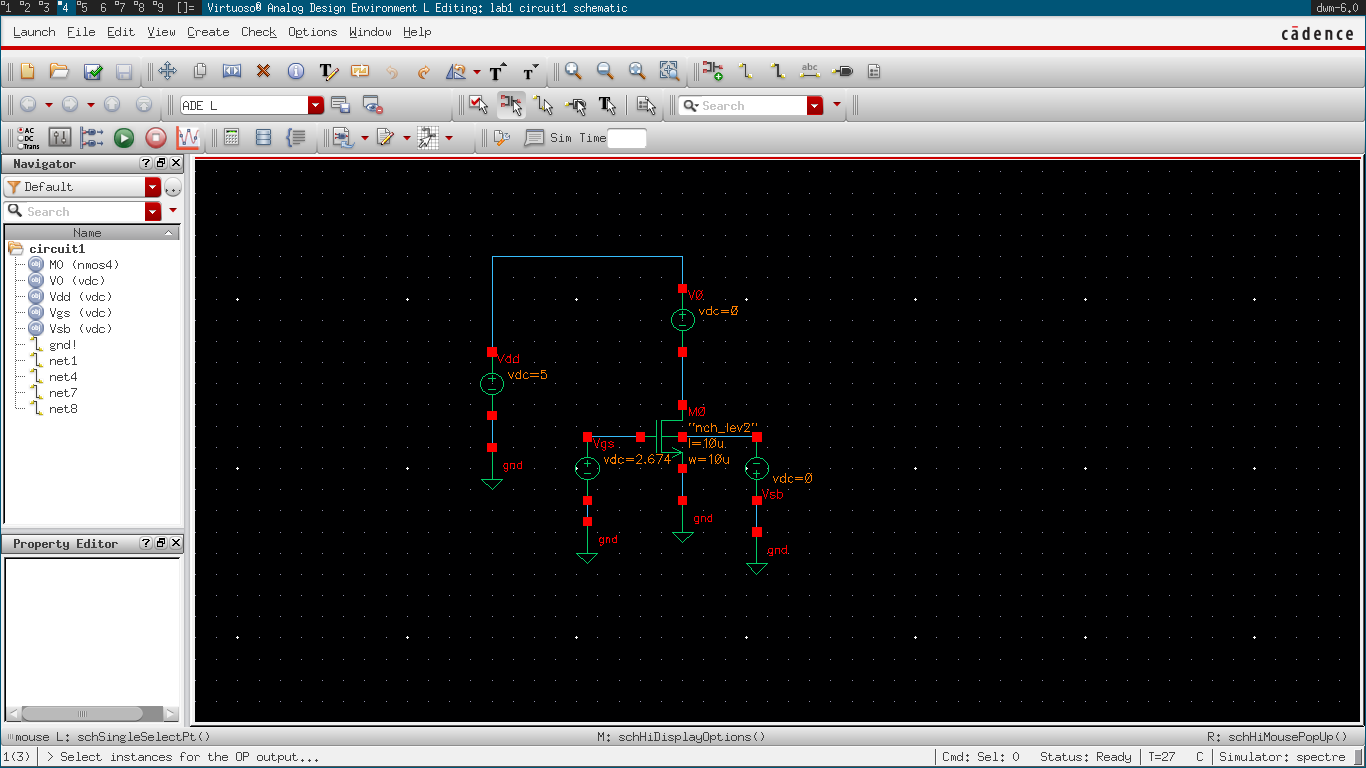
\includegraphics[scale=0.3]{./images/circuit1.PNG}
	\caption{Circuit for Simulation 1}
	\label{fig:circuit1}
\end{figure}

\FloatBarrier

The value of $V_{GS}$ for which $I_{D} = 500$\si{\micro\ampere} is listed in table (\ref{tab:sim1_results}).
$g_{m}$ is determined from a DC operating point analysis in Virtuoso as well as from the plot in figure (\ref{fig:id_vs_vgs}).

\FloatBarrier

\begin{figure}[h!]
	\centering
	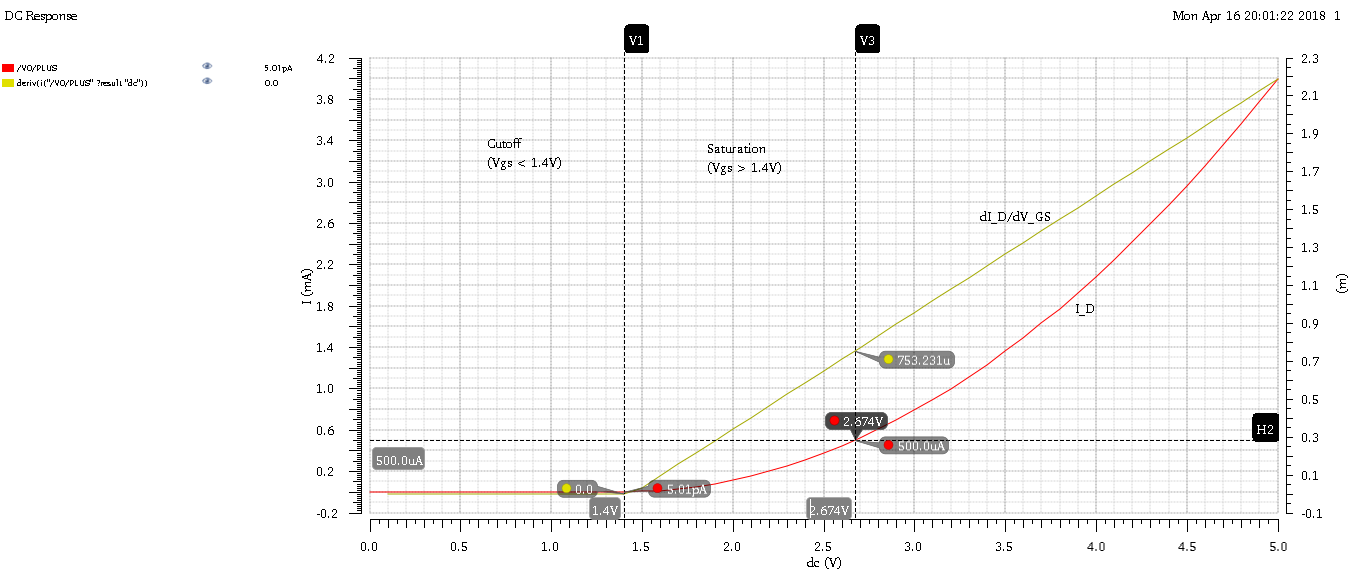
\includegraphics[scale=0.45]{./images/500ua_point.PNG}
	\caption{$I_{D}$ and $\frac{\partial I_{D}}{\partial V_{GS}}$ versus $V_{GS}$ for NMOS}
	\label{fig:id_vs_vgs}
\end{figure}

\FloatBarrier

It should be noted that the transistor is always in saturation when it is not in cutoff since $V_{DS} = 5$\si{\volt} and $V_{GS} < 5$\si{\volt}, which implies $V_{GS} - V_{t} < V_{DS}$.
By definition, $g_{m} = \frac{\partial I_{D}}{\partial V_{GS}}$.
So, $g_{m}$ can be determined from the graph at the point when $I_{D} = 500$\si{\micro\ampere}.

\FloatBarrier

\begin{table}[h!]
	\centering
	\caption{Simulation 1 Results}
	\label{tab:sim1_results}
	\csvautotabular{./tables/sim1_results}
\end{table}

\FloatBarrier
